\chapter{Mechanical Design}
\label{chap:mech_design}
As pointed out in the previous chapter, the major task of this project was to devise an efficient mechanical
design. Two different designs both based on extension springs were looked into. 
This chapter describes them and the motivation behind choosing the final design to be fabricated.

\section{Design 1}
Write general description of design 1 here.
\subsection{Energy pumping}
\begin{figure}[!h]
\centering
%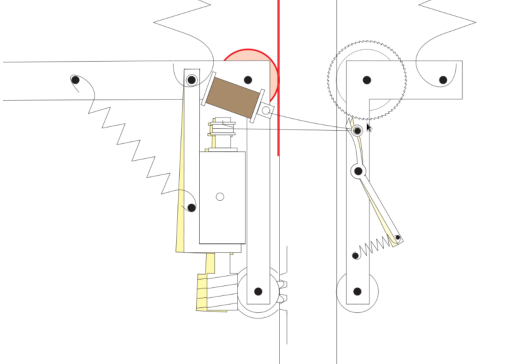
\includegraphics[scale=0.5]{fig/seth_design.pdf}
\caption{Winding motor with pulley on the leg}
\label{fig:3_pratik_design}
\end{figure}
Fig. \ref{fig:3_pratik_design} shows the pulley mechanism for storing energy in the large central spring.
The winding motor is placed upon the platform which can be called as the larger mass M of the two mass
system. A winch connects the motor to the same platform passing over the pulley on the lower leg. Thus, as
the motor rotates, it pulls the platform (and itself) downwards while extending the spring above it. 
A few points to note about the energy pumping design are,
\begin{enumerate}
\item
The motor has to move a distance twice that of the extension of the spring. This is
especially important when we look at the timescales over which we have to extend the spring, these are around
200-300 msecs. A larger distance in smaller time results in a large $\omega$ for the motor which translates
to a smaller available torque. This neccesitates a larger motor which can provide this torque. 
\item
The large mass of the platform (M) is helping in the extension of the spring and hence the torque required
for the winding motor reduces.
\item
It has to be ensured that the winding winch does not slip over the pulley when the platform is suddenly released from
the constraint. At the same time, the winch must be free enough so as not to hinder the movement of the platform after
the release.
\end{enumerate}

\subsection{Constraint}
\begin{figure}[!h]
\centering
%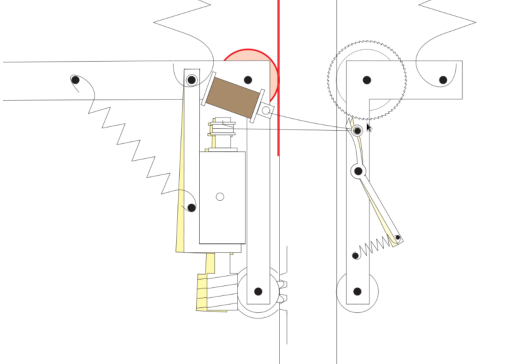
\includegraphics[scale=0.5]{fig/seth_design.pdf}
\caption{Constraint for the pulley}
\label{fig:3_pratik_constraint}
\end{figure}
Fig. \ref{fig:3_pratik_constraint} shows the constraint mechanism for the pulley. It consists of a hatch connected to
the lower leg with a torsional spring. The toothed part of the pulley is free to move in the clockwise direction (thus
compressing the torsional spring every time). The lower part of the leg is cylindrical with a top flange which matches
the top face of the cylindrical bushing shown inside the main leg. Thus the lower leg can move only up. The protruding
portion of the main leg prevents the hatch from moving in the clockwise direction, thus constraining the pulley from
rolling back in the anti-clockwise direction.
Salient points of this part are,
\begin{enumerate}
\item
The diameter of the lower leg is expected to be around 2-3 cms and it is difficult to fabricate the hatch on such
a small surface.
\end{enumerate}

\subsection{Using the impact for energy release}
This design is unique because it utilizes the impact force ($m\:v_{touch-down}$) to release the stored energy in the main
spring. Visualize the lower leg impacting on the ground. This results in the hatch (which is holding the pulley from
moving back) impacting against the protrusion of the main leg. Since the impact force is easily larger than the torsional
spring force, the hatch closes and the lower leg goes inside the main leg thus enabling free rotation of the pulley. There
is a compression spring inside the main leg connected to the lower leg which gets compressed while this happens. It is
responsible for pushing the lower leg back outside after $t_{liftoff}$.

\section{Design 2}
\begin{figure}[!h]
\centering
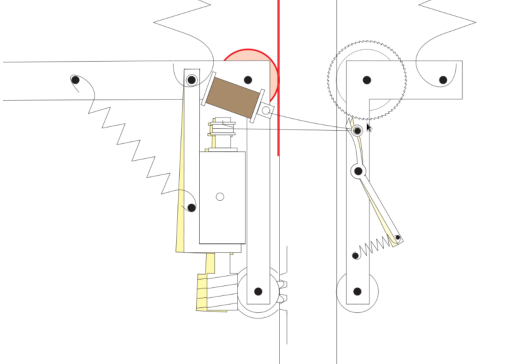
\includegraphics[scale=0.5]{fig/seth_design.pdf}
\caption{Rack and pinion on the leg with the drive motor}
\label{fig:3_seth_design}
\end{figure}

\subsection{Energy pumping}
The leg consists of a rack on one of its sides. A single dual shaft motor in a sleever is used to drive the pinion
on this rack as
well as pull the paul to free the ratchet. This motor consists of a string attached to a friction pulley on the shaft.
A friction pulley is a device whose coupling is dependent upon the speed of the relative motion between the two surfaces.
Thus, the motor can pull the paul only beyond a certain $\omega$. Below this speed, the paul spring is enough to
engage it with the ratchet.

\subsection{Constraint} 
The platform and the ratchet are rigidly connected to a band drive which rolls along
the length of the leg. This ensures that contact of the roller inside the band drive and the leg is maintained at all
times. Since the ratchet is rigidly connected to the platform, both can only move together i.e. only when the paul is
pulled by the drive motor. 

\subsection{Energy release}
This design uses an electromechanical system to release energy. After sensing the impact through a touch switch located
below the leg, we can use a voice coil actuator to slack the string attached to the paul. This brings in the pull
back spring attached to the sleeve into the picture and it prompty pulls the sleeve away from the rack.
\textbf{Not sure about this part.}

\section{Modifications}





